Given the puzzling results of the immunolabeling experiment performed on 6 March, a second immunolabeling experiment was carried out to answer two lingering questions:
1. Do the naked Au spheres and fully labeled spheres generate nonspecific contrast enhancement by binding to the coverslip?
2. Does permeabilizing the cells with Triton-X so that the cells can be stained with Sytox Green and phalloidin allow the gold nanospheres to diffuse into, but not out of, the cells, leading to nonspecific contrast enhancement?
To address these questions, the gold-labeled preparations from the previous experiments were repeated without permeabilization and two new preparations were added, consisting of coverslips without cells and with gold labeling agents.

\section{Structure of the Immunolabeling Experiment}
\label{structureoftheimmunolabelingexperiment}

6 preparations and their expected outcomes are described in \autoref{tab:3AprilPrepTable}. The labeling procedure was changed to remove the permeabilization (and the fluorescent stains, as they cannot label without the permeabilization). Full details are in \autoref{The3AprilImmunolabelingProtocol}, but in brief, the procedure was:

\begin{enumerate}
\item Fix cells with paraformaldehyde

\item Add primary antibody if appropriate for a given preparation

\item Add appropriate secondary labeler
\end{enumerate}

Since the permeabilization was removed, the Sytox Green and phalloidin cannot label the intracellular structures; as a result the only fluorescence contrast would come from the AP124F. The permeabilization concerns were specific to the 2Au-labeled preparations, so no confocal fluorescence imaging was performed, only OCM imaging, again using 5 $500\,\mu\mathrm{m}\,\times\,500\,\mu\mathrm{m}$ fields of view.

\rowcolors{1}{}{lightgray} 
\begin{table}[htb]
\caption{Description of the six preparations used in the 3 April immunolabeling experiment; each preparation is described by whether the primary antibody (MAB1999) was added, what secondary labeler (AP124F PEGylated to Au nanospheres or naked Au nanospheres) was added, and whether or not an increase was expected in backscattering.}
\begin{minipage}{\linewidth}
\setlength{\tymax}{0.5\linewidth}
\centering
\small
\begin{tabular}{lp{2cm}p{2cm}p{2cm}} \toprule
Preparation Name&Primary Antibody?&Secondary Labeler?&+Scattering Expected?\\
\midrule
Cells Only&No&No&No\\
Au&No&Naked Au&Yes\\
2Au&No&OPAb-Au-PS&No\\
1--2Au&Yes&OPAb-Au-PS&Yes\\
Coverslip-Au&No&Naked Au&Yes\\
Coverslip--2Au&No&OPAb-Au-PS&No\\

\bottomrule

\end{tabular}
\end{minipage}
\label{tab:3AprilPrepTable}
\end{table}

The results for the cells only sample should be the same as in the 6 March experiment. If permeabilization is causing gold spheres to become trapped in the cells, the voxels occupied by cellular material in the Au, 2Au, or 1-2Au samples should scatter less than the equivalent voxels for the permeabilized cells. As for the coverslips, the protein and PEG coating on the 2Au should prevent it from binding to the coverslip, resulting in very low scattering. Given the results from 6 March, the naked Au is expected to bind quite strongly to the coverslip via van der Waals forces, resulting in high scattering.

\begin{figure}[p]
\centering
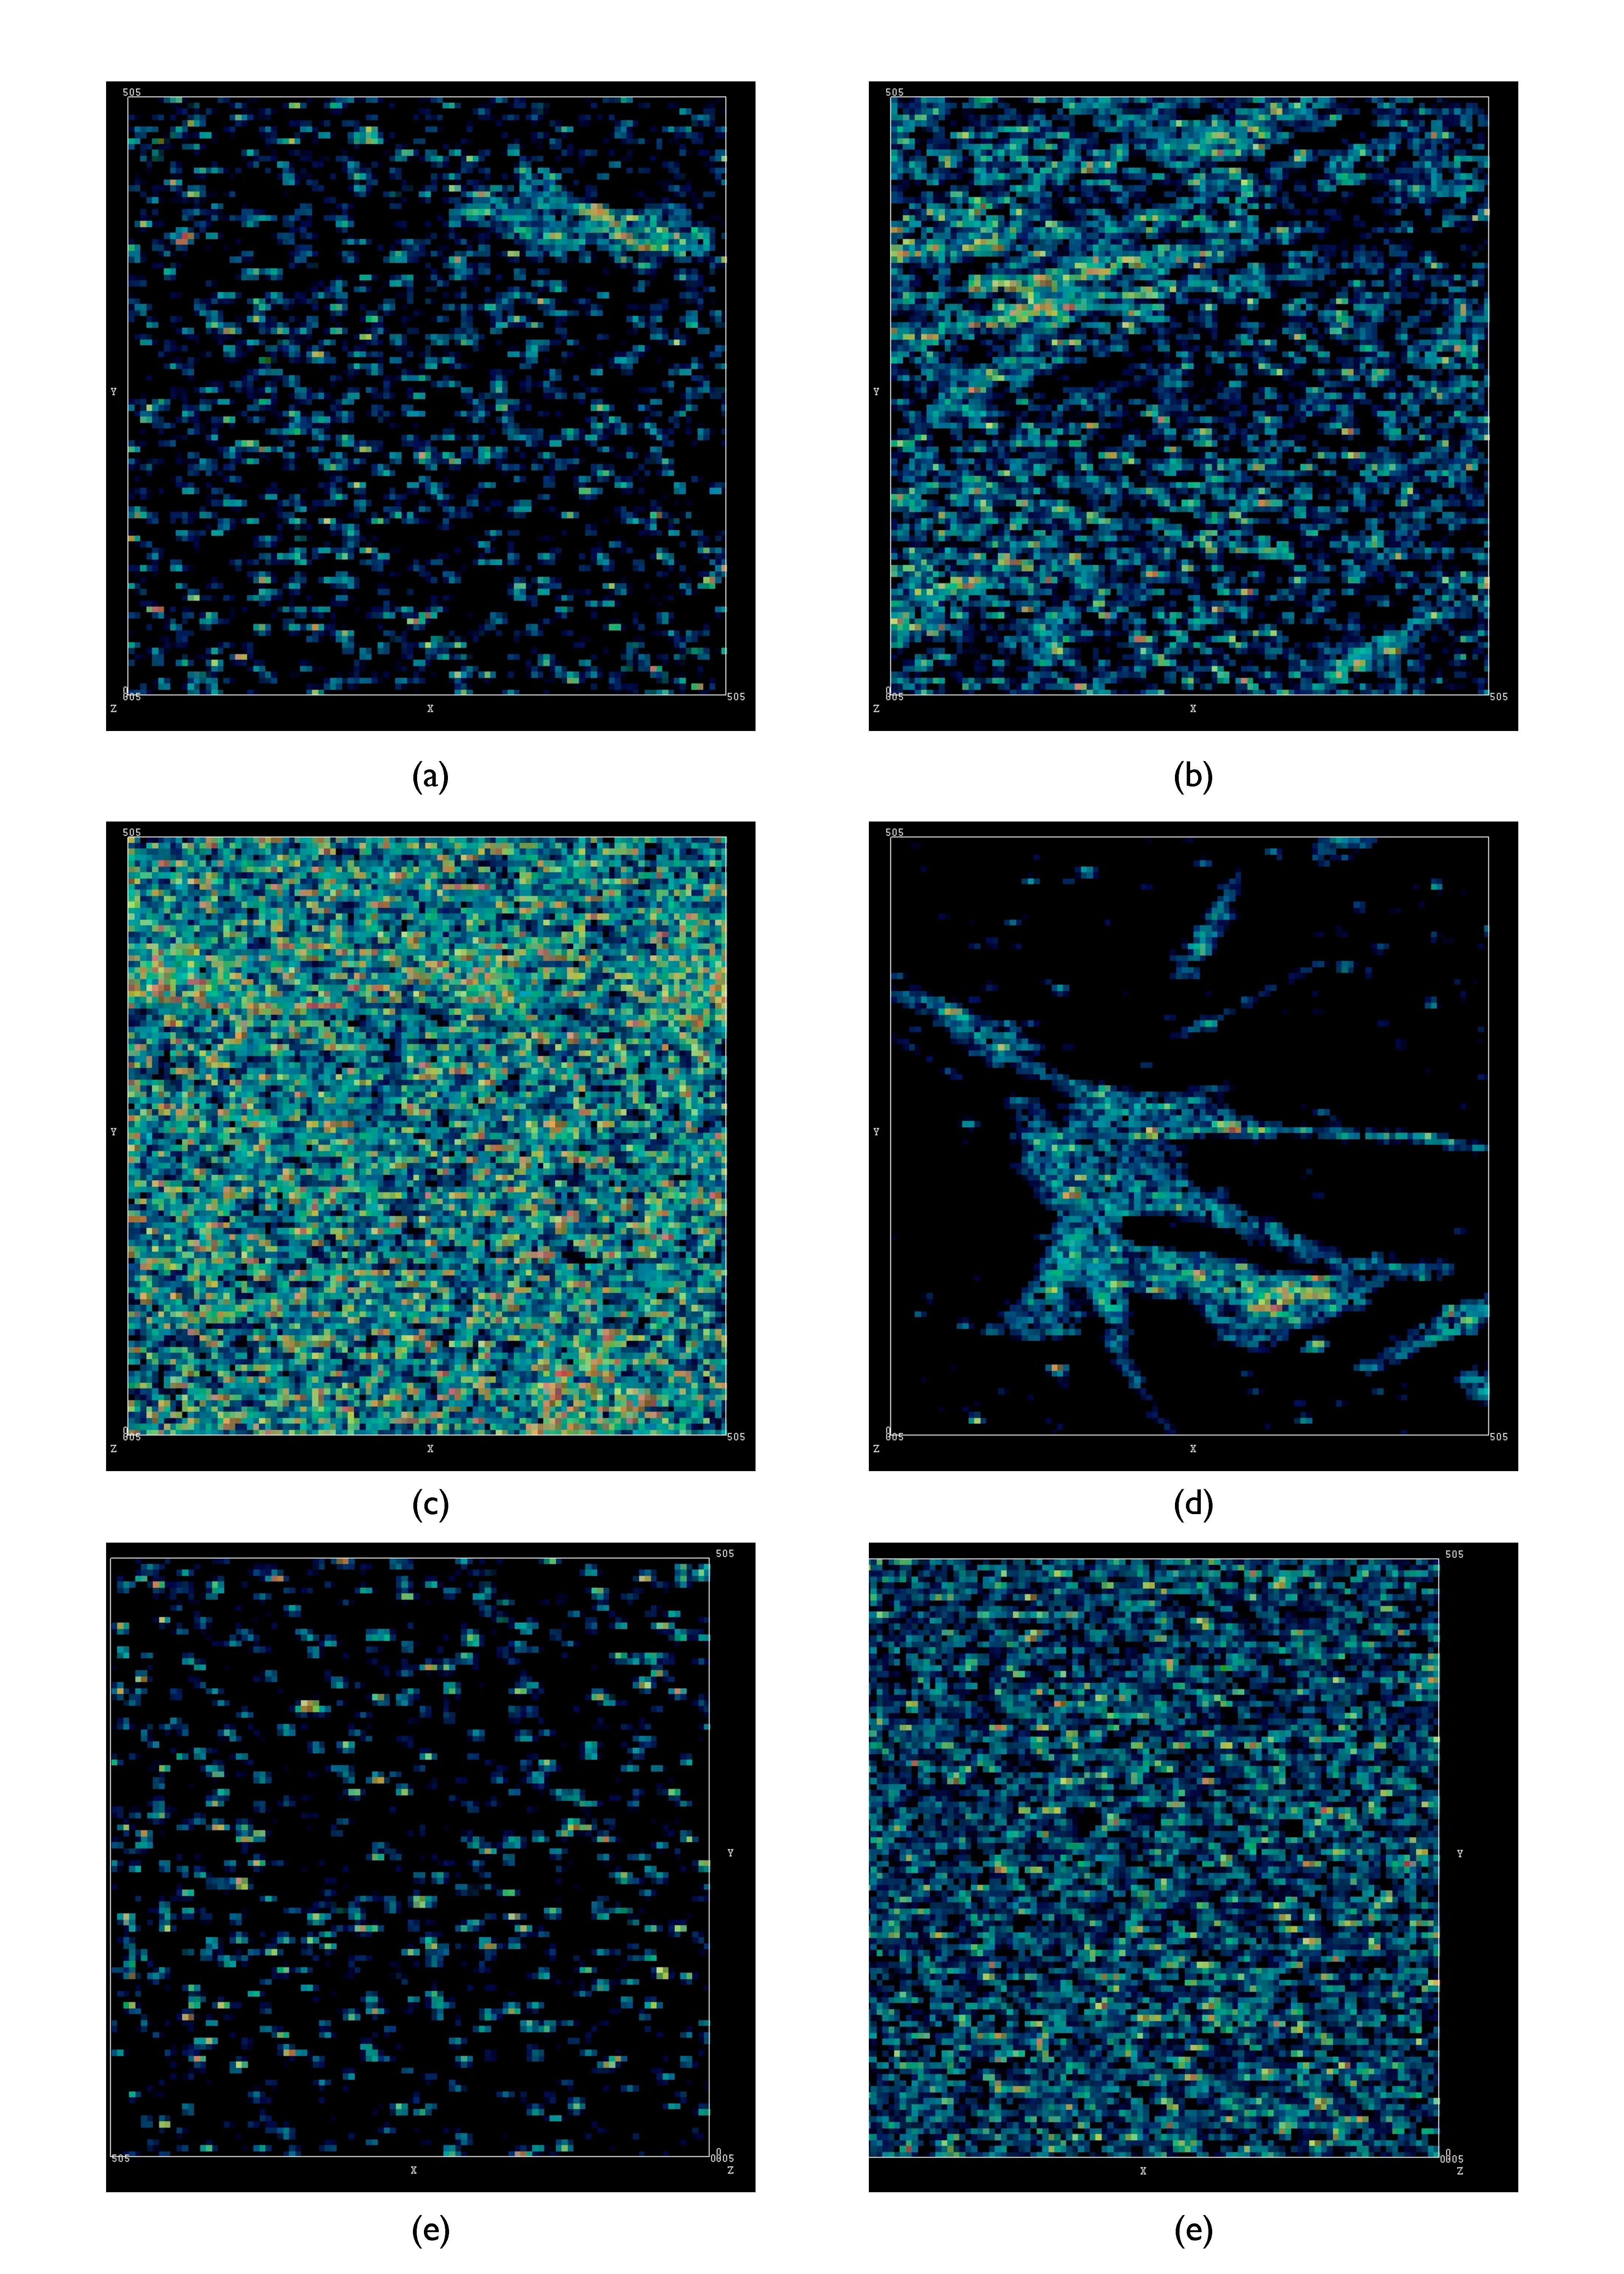
\includegraphics[keepaspectratio,width=\textwidth,height=0.75\textheight]{3aprOCMreps.pdf}
\caption{Representative OCM images of the 6 preparations from the 3 April immunolabeling session. Images correspond to preparations: (a) 1--2Au; (b) 2Au; (c) Au; (d) Cells only; (e) Coverslip--2Au; (f) Coverslip-Au.}
\label{aprocmreps}
\end{figure}

\section{Results of the Immunolabeling Experiment}
\label{resultsoftheimmunolabelingexperiment}

Representative images from the OCM are shown in \autoref{aprocmreps}. There is a marked difference between the permeabilized and non-permeabilized preparations for the 1--2Au and 2Au preparations. First, cellular features are much more easily distinguished. This is likely due to the fact that the cells were allowed to grow on the coverslips for a shorter period than the previous set of cells, leading to a lower level of cell coverage and thus keeping most cells isolated. This lower cell density is harder to observe in the naked Au image due to the high amount of background from the Au nanospheres binding to the coverslip. The coverslip binding is demonstrated directly by the Coverslip-Au preparation: the binding is fairly homogenous and quite high. The Coverslip--2Au preparation also shows some scatterers present in the volume, though far fewer than the Coverslip-Au preparation. This is further evidence of the successful protection of the gold nanospheres by the PEG-SH and OPAb.

The same sum-of-voxels-squared analysis method was used on this set of images; a chart of those values is in \autoref{aprsos}. There is again clear contrast enhancement and again the naked-Au-labeled cells are quite far above the rest of the samples. This time, however, the scattering from the 2Au-labeled cells is greater than the scattering from the 1--2Au-labeled cells in a statistically significant manner. This is exceptionally puzzling, as it suggests that the presence of primary antibody \emph{decreases} the amount of nonspecific binding quite considerably, either in conjunction with or instead of increasing the amount of specific binding. Clearly, more work must be done to understand this phenomenon.

\begin{figure}[htbp]
\centering
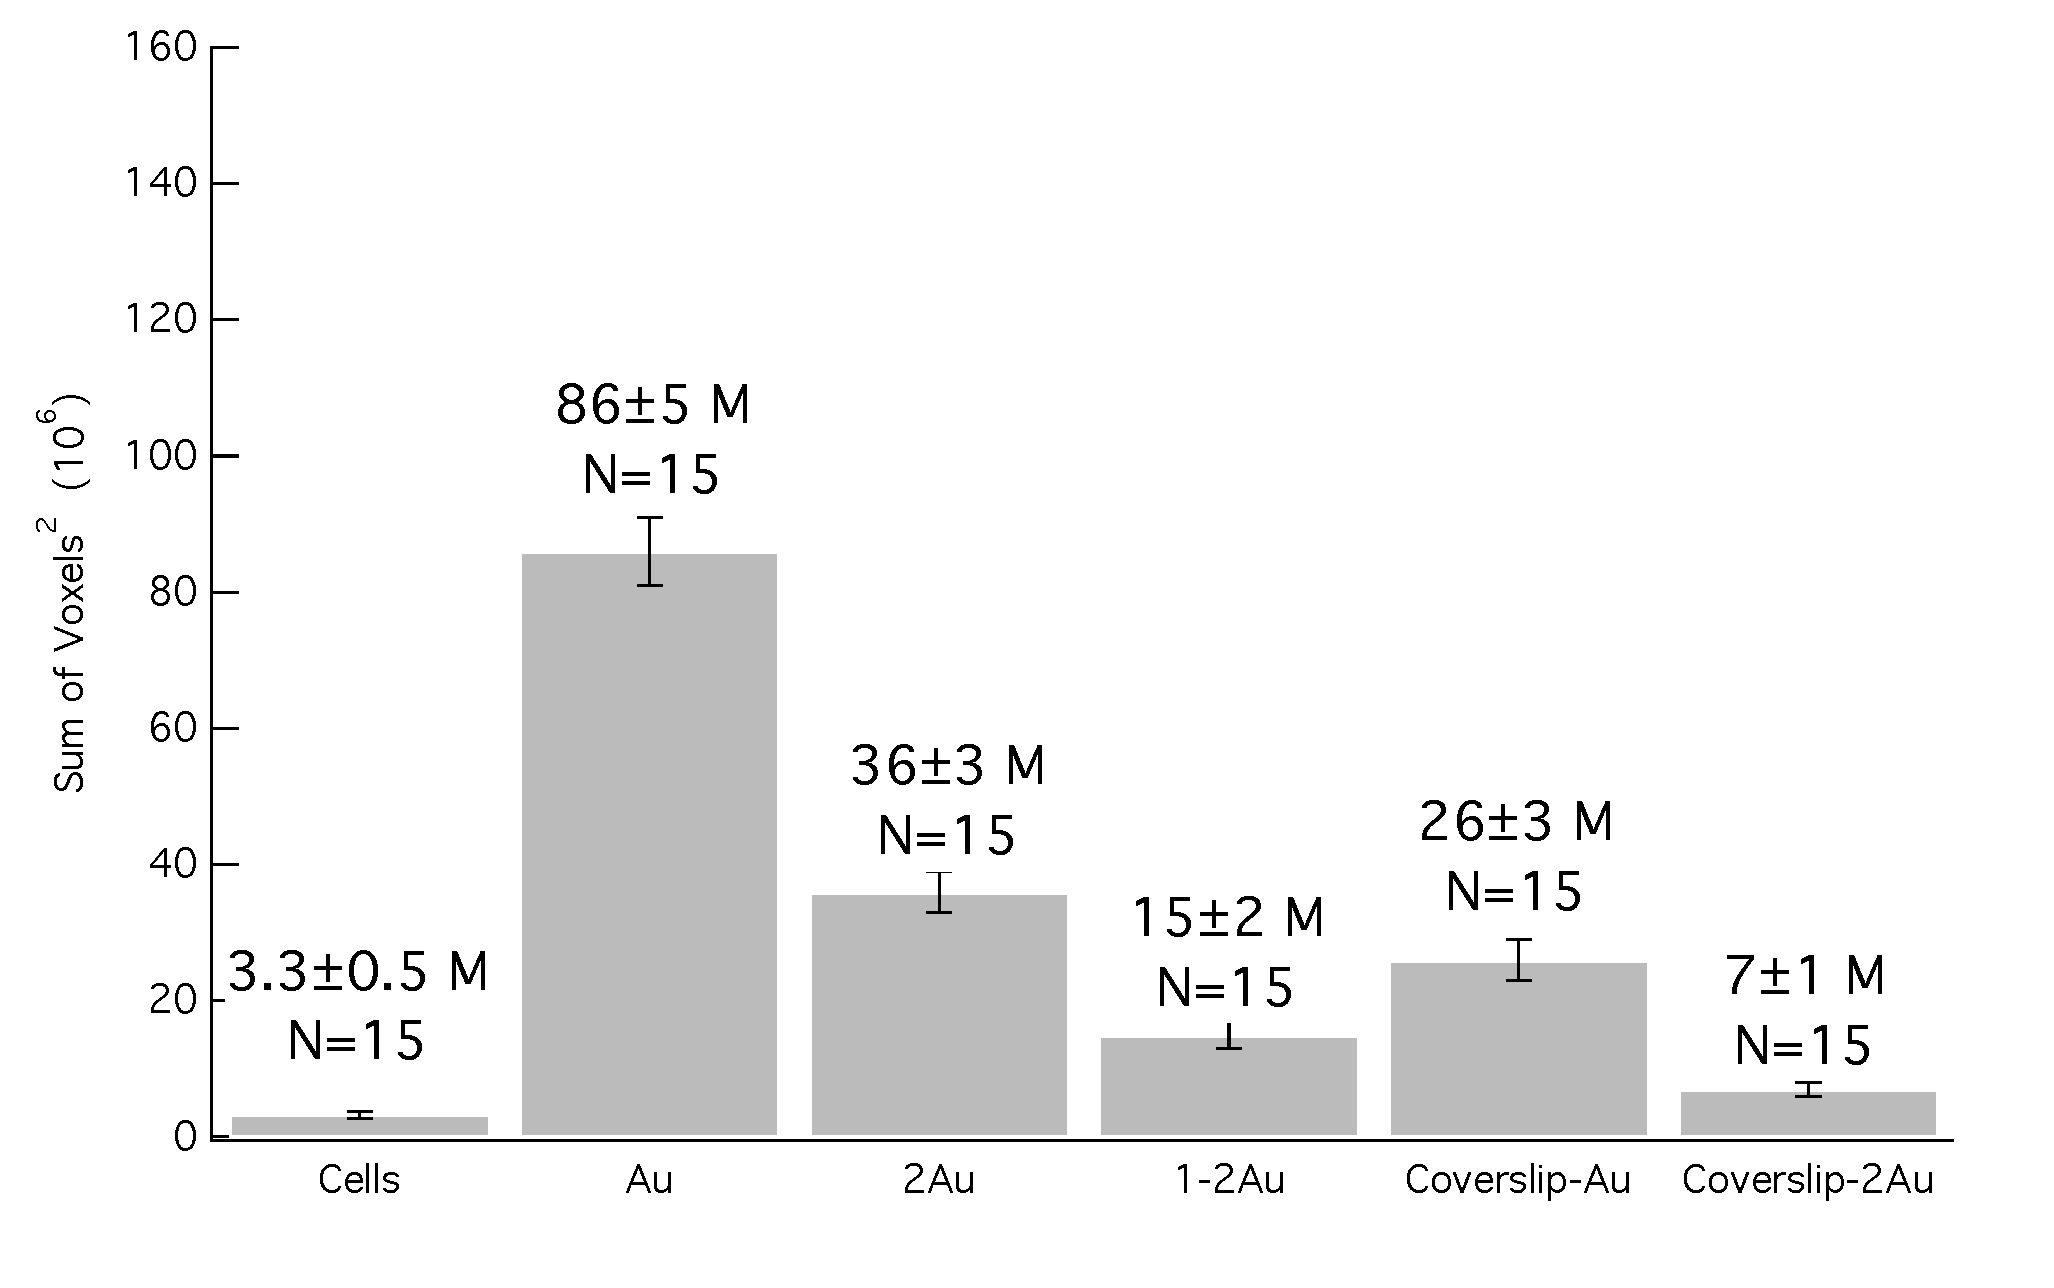
\includegraphics[keepaspectratio,width=\textwidth,height=0.75\textheight]{3aprSOSgraph.pdf}
\caption{Plot of the mean of the sum of voxel values squared for all preparations. Values are formed by taking the mean and standard error of sum of voxel values squared for each image corresponding to a given preparation.}
\label{aprsos}
\end{figure}

Determining whether or not the permeabilization had an effect is something of a difficult business. Since the cells were at different stages of confluence, the two immunolabeling sessions cannot be compared directly. Rather, some normalization must take into account the different amount of cell coverage. It is not sufficient to simply divide by the scattering from the cells, as that ignores the binding of the spheres to the coverslip. Rather, let us approximate the coverslip and cells as a 2D grid, each pixel of which is either occupied completely by cell or completely by coverslip. Each pixel then contributes, on average, some amount of scattering depending on whether it is cell or coverslip; this amount is determined both by binding affinity and the scattering cross section of the scatterer. The sum of voxels squared, $S_{\mathrm{voxels}^2}$ can then be determined on average as a function of the fraction $F$ of the viewing region covered by cell as
\[S_{\mathrm{voxels}^2}=S_{\mathrm{Coverslip}}(1-P)+S_{\mathrm{Cell}}P\]
where $C_{\mathrm{Coverslip}}\mathrm{\ and\ }C_{\mathrm{Cell}}$ are the scattering from a view of view filled by coverslip or cellular materials labeled with the secondary labeler in question, respectively. We can determine $C_{\mathrm{Coverslip}}$ from the coverslip binding sum of voxels squared; since they are taken at $P=0$, $S_{\mathrm{voxels}^2}=C_{\mathrm{Coverslip}}$. From \autoref{aprsos}, $C_{\mathrm{Coverslip,\,Au}}=2.6\pm0.3\times10^7$ and $C_{\mathrm{Coverslip,\,2Au}}=7\pm1\times10^6$. To determine whether or not reducing the permeabilization had an effect, we need to determine $C_{\mathrm{Cell}}$ for Au and 2Au. We now see that we cannot simply divide by the scattering of the cells, which is $S_{\mathrm{Cells\ Only}}=C_{\mathrm{Cell,\,No\, Label}}P$, because that would give
\[S_{\mathrm{norm}}=\frac{C_{\mathrm{Coverslip}}(1/P-1)+C_{\mathrm{Cell}}}{C_{\mathrm{Cell,\,No\, Label}}}\]
which still has $P$ dependence. However, if we first normalize by subtracting $C_{\mathrm{coverslip}}$, we get
\begin{equation}
S_{\mathrm{norm}}=\frac{S_{\mathrm{voxels}^2}-C_{\mathrm{Coverslip}}}{S_{\mathrm{Cells\ Only}}}=\frac{-C_{\mathrm{Coverslip}}+C_{\mathrm{Cell}}}{C_{\mathrm{Cell,\,No\, Label}}}
\label{eq:normalization}
\end{equation}
This is sufficient to perform comparisons between the two immunolabeling sessions, as it does not depend on $P$ at all; $C_{\mathrm{Cell}}$ could be calculated with sufficient image analysis, but generating a large enough dataset to adequately calculate it is beyond the scope of of the studies performed. The results of performing this normalization are shown in \autoref{normalizedsvx2}. For the naked Au the difference is actually the opposite of expected: the permeabilization decreases the amount of scattering per cell coverage; however, the uncertainties on this calculation are quite large, and consequently the difference is statistically consistent with 0. The same hold for the 2Au preparation, though the uncertainties are somewhat smaller and it shows the expected decrease. 1--2Au is the only preparation with a statistically significant difference, and the difference is quite large. Therefore, though there is a large amount of statistical uncertainty, permeabilization does appear to reduce the amount of scattering, which implies that gold spheres are getting inside of the cells. As this is undesirable, and the OCM imaging does not benefit from the fluorescent stains, permeabilization should not be used in future immunolabeling experiments.

\begin{figure}[htbp]
\centering
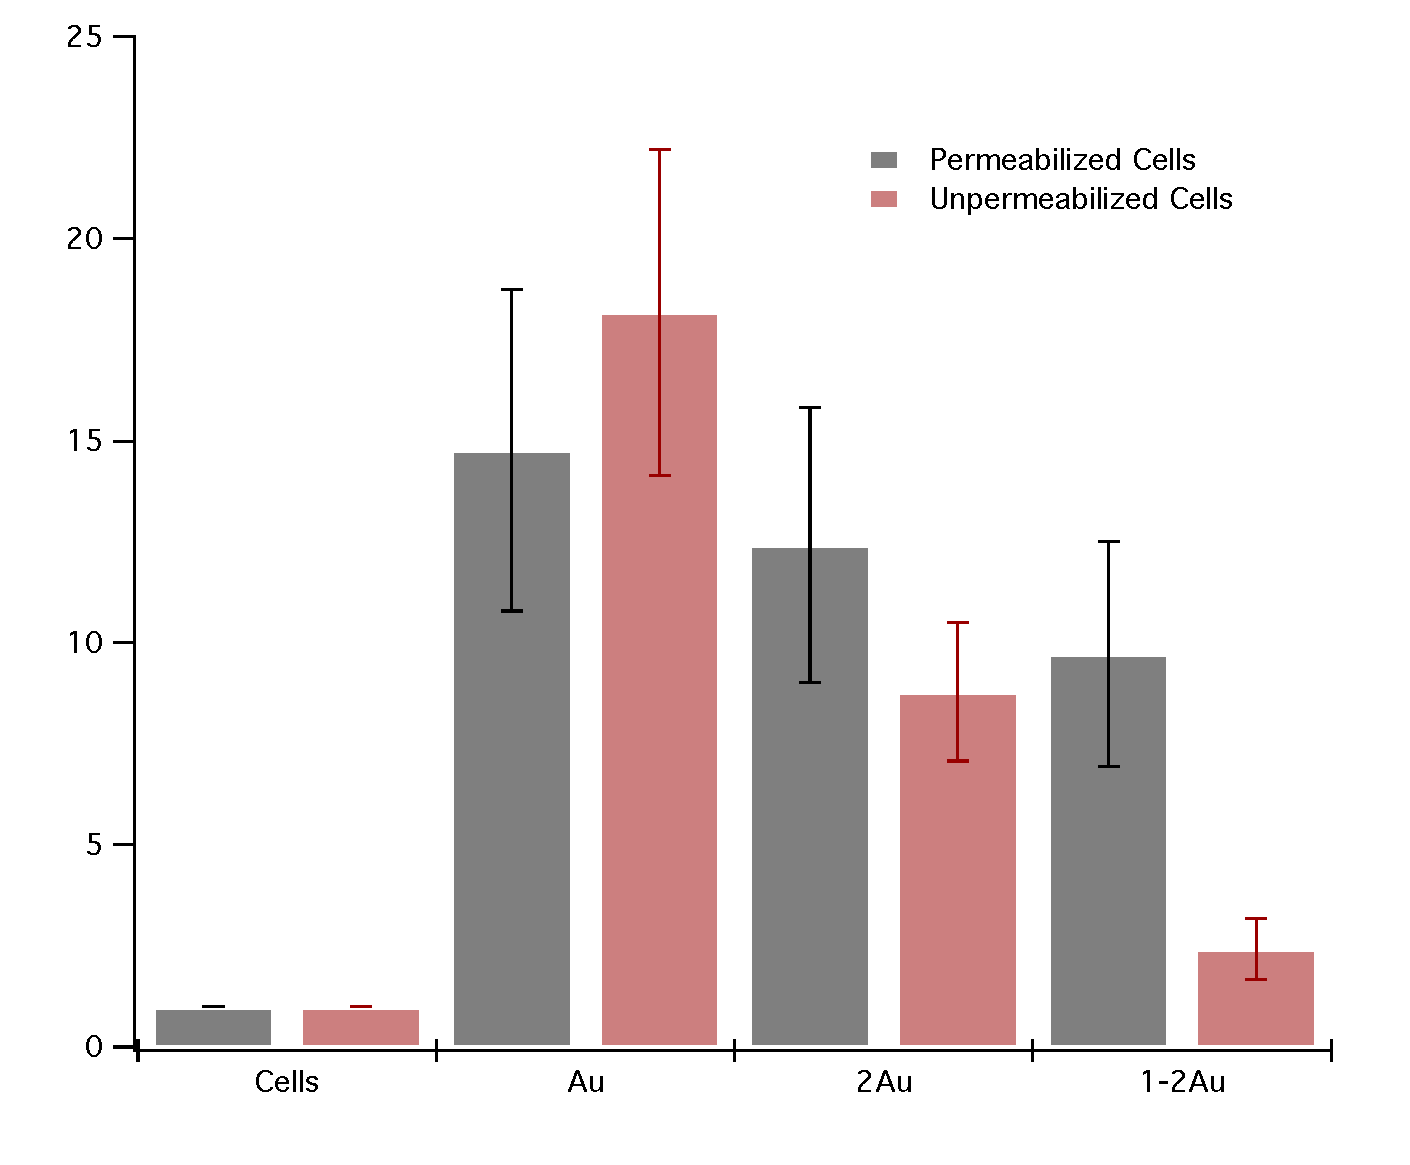
\includegraphics[keepaspectratio,width=\textwidth,height=0.75\textheight]{NormalizedSvx2.pdf}
\caption{Sum of voxel values squared for gold-labeled preparations and cells, normalized using \autoref{eq:normalization}.}
\label{normalizedsvx2}
\end{figure}



As for van der Waals binding, both the Coverslip-Au and the Coverslip--2Au preparations indicate that van der Waals interactions are occurring between the coverslip and the gold, even when it's well-protected by the PEG. Furthermore, there must be strong van der Waals interactions occurring between the cell and the 2Au; though some non-specificity of the secondary antibody is expected, the extent to which the unpermeabilized 2Au preparation displays nonspecific binding to the cell is too large to simply be explained by poor localization of the protein. The high polarizability of the gold creates the potential for strong van der Waals forces, and it may be the case that despite the \ensuremath{\sim}7nm dielectric coating, a strong dipole can be induced in the gold.
